\documentclass[10.5pt,twocolumn]{jbuaa}
\newcommand*\circled[1]{\tikz[baseline=(char.base)]{
            \node[shape=circle,draw,inner sep=1pt] (char) {#1};}}
\usepackage{amsmath}  
\usepackage{float}   
\usepackage[numbered,framed, autolinebreaks]{mcode}
%取消英文连词符
% \tolerance=1
% \emergencystretch=\maxdimen
% \hyphenpenalty=10000
% \hbadness=10000
\usepackage{enumitem}
\usepackage{bm}

\newcommand\mycolorRed[1]{{\color{red}#1}}
\newcommand\mycolorYellow[1]{{\color{yellow}#1}}
% \newcommand*\mycolorRed{\color{red}}

%%%????? 公式中字体的定义尺寸为 10 磅,上标/下标 68%,次下标/上标 42% ?????? 
\DeclareMathSizes{10.5}{10}{6.8}{4.2}
%%%% 本示例中带单位的数据采用的是siunitx来生成,好像默认与公式同样大小的字体,所以数字在正文中会小一些
%%%% 行文中普通数字大小为10.5pt,公式里或者用siunitx生成的数字则会是10pt,多少有点不协调。

%%%设置公式前后距离,差不多近似
\setlength{\abovedisplayskip}{2.5mm}
\setlength{\belowdisplayskip}{2.5mm}


\usepackage{tabu}
\usepackage{longtable}
\usepackage{makecell}
\renewcommand\cellgape{\Gape[-3pt][-3pt]}


%%%%%%%%%%%%%%%%%%%%%%%%%%%%%%%%%%%%%%%%%%%%%%%%%%%%%%%%%%%%%%%%
%      文章正文
%%%%%%%%%%%%%%%%%%%%%%%%%%%%%%%%%%%%%%%%%%%%%%%%%%%%%%%%%%%%%%%%
\begin{document}
%%%%%%%%%%%%%%%%%%%%%%%%%%%%%%%%%%%%%%%%%%%%%%%%%%%%%%%%%%%%%%%%
% 标题,基金项目,作者,通信地址定义
%%%%%%%%%%%%%%%%%%%%%%%%%%%%%%%%%%%%%%%%%%%%%%%%%%%%%%%%%%%%%%%%
\title{
\vspace{1cm} \erhao\hei 基于启发式算法的标定最优化问题 \vspace{-0.2cm}
}

\author{
\sihao\fang 吕艺 \makebox{$^{\text{1}}$},冯伟琪 \makebox{$^{\text{2}}$}\\[0.1cm]
\liuhao (1.~~上海交通大学~~电子信息电气工程学院,上海~~200240;2.~~上海交通大学~~电子信息电器工程学院,上海~~200240)
}

\date{}  % 这一行用来去掉默认的日期显示
%%%%%%%%%%%%%%%%%%%%%%%%%%%%%%%%%%%%%%%%%%%%%%%%%%%%%%%%%%%%%%%%
% 奇数页页眉
%%%%%%%%%%%%%%%%%%%%%%%%%%%%%%%%%%%%%%%%%%%%%%%%%%%%%%%%%%%%%%%%
\fancyhead[CO]{{\footnotesize 工程建模与仿真}}            %请在这里写出第一作者以及论文题目
%%%%%%%%%%%%%%%%%%%%%%%%%%%%%%%%%%%%%%%%%%%%%%%%%%%%%%%%%%%%%%%%
%%%%%%%%%%%%%%%%%%%%%%%%%%%%%%%%%%%%%%%%%%%%%%%%%%%%%%%%%%%%%%%%
%  显示title,并设页码为空(按杂志社要求)
%%%%%%%%%%%%%%%%%%%%%%%%%%%%%%%%%%%%%%%%%%%%%%%%%%%%%%%%%%%%%%%%
%%%%%%%%%%%%%%%%%%%%%%%%%%%%%%%%%%%%%%%%%%%%%%%%%%%%%%%%%%%%%%%%
%      中文摘要
%%%%%%%%%%%%%%%%%%%%%%%%%%%%%%%%%%%%%%%%%%%%%%%%%%%%%%%%%%%%%%%%
\CKeyword{工程标定;遗传算法;三次样条插值}
\twocolumn[
  \begin{@twocolumnfalse}
  \maketitle
\begin{CAbstractJBUAA}
本文首先引入一个测量装置在大规模制造中的标定问题,介绍工程实践中标定成本问题。然后,本文介绍了多项式插值、三次样条差值、$Hermite$插值三种常见的插值方法。针对标定最优化问题,本文给出了遗传算法和模拟退火算法的算法原理。并利用两种算法,对该标定问题进行优化求解。最后,本文针对两种启发式最优化模型进行算法性能分析,并研究相关参数对优化结果的影响。
\end{CAbstractJBUAA}
\begin{center}
\parbox{\textwidth}{
\setlength{\parindent}{1em}
{
\centering\sihao\textbf{Calibration Optimization Problem Based on Heuristic Algorithm}\\
} 
\vspace{-1.2mm}
\begin{center}
\wuhao Yi Lyu\makebox{$^{\text{1}}$}, Vic Feng\makebox{$^{\text{2}}$}\\[-0.1cm]
\liuhao{1. School of Electrical and Engineering, Shanghai Jiao Tong University, Shanghai 200240, China;\\
2. School of Electrical and Engineering, Shanghai Jiao Tong University, Shanghai 200240, China;}
\end{center}

\wuhao
{
\textbf{Abstract:} 
Initially, a calibration problem of measurement apparatuses in massive manufacturing is raised in order to draw the calibration cost problems in engineering practices. Next, the article introduces three common interpolation methods--Polynomial Interpolation, Cubic Spline Interpolation and Hermite Interpolation. To solve the calibration optimization problem, we start by explaining two algorithms—Genetic Algorithm and Genetic Annealing Algorithm and then apply them to optimize the result. Finally, we analyze these two algorithms’ performances and the impacts of different parameters on the final optimized result.

\textbf{Key words:} Engineering Calibration; Genetic Algorithm; Cubic Spline Interpolation}
}
\end{center}

%%%%%%%%首页角注
%\positiontextbox{2.0cm}{25cm}{
%\noindent\rule{4cm}{.5pt}\\[0.5ex]%
%\hspace*{1em} \liuhao \linespread{0.8}\selectfont
%\parbox{\textwidth}{%
%\hei\makebox[\widthof{\makebox{*}收}][r]{收}稿日期: 2015-**-**; 录用日期: 2015-**-**; 网络出版时间:(此行信息已填) \\%
%\hei\makebox[\widthof{\makebox{*}收}][r]{网}络出版地址: (已填)\\
%\hei\makebox[\widthof{\makebox{*}收}][r]{基}金项目:国家自然科学基金(基金号~12345678);中国博士后科学基金(基金号~87654321)(注意:国家级基金放前,地方级放后)\\
%\hei\makebox[\widthof{\makebox{*}收}][r]{\makebox{*}通}信作者:E-mail:bhxb@buaa.edu.cn\\ \\
%\hei\makebox[\widthof{\makebox{*}收}][r]{引}用格式:(可不填)
%}}
  \end{@twocolumnfalse}
]
%%%%%%%%%%%%%%%%%%%%%%%%%%%%%%%%%%%%%%%%%%%%%%%%%%%%%%%%%%%%%%%%
%  正文由此开始-------------------------
%%%%%%%%%%%%%%%%%%%%%%%%%%%%%%%%%%%%%%%%%%%%%%%%%%%%%%%%%%%%%%%%
%%%%%%%%%%%%%%%%%%%%%%%%%%%%%%%%%%%%%%%%%%%%%%%%%%%%%%%%%%%%%%%%
\wuhao 
%  分栏开始

%%%%%!!!!!正文在第一页两栏分别合适位置插入 \enlargethispage{-3.3cm},给首页跨双栏脚注留空间,大小需要结合前面位置和高度手动设置!!!!!
%%%%%%%%%%%%%%%%%%%%%%%%%%%%%%%%%%%%%%%%%%
\section{引言}
很多大规模制造的电子产品中包含有带测量功能的模块(测量装置),用于监测某种物理量,比如环境温度、压力或光照强度等。任何测量装置在制造时一般都要经过标定。

本课题假定一种测量装置。为便于理解,假定被测物理量为环境温度,可测范围是$-20^\circ$C至$69^\circ$C。所用核心传感器的输入-输出特性有明显非线性,且个体差异性比较大。课题要求为该装置设计一种标定工序的方案,适合大规模高效率制造\citeBUAA{Paper1}。
\subsection{标定过程分析}
结合我们课堂上提到的弹簧测力器的案例,我们可以将其与本篇报告中所要解决的案例形成类比。在制作弹簧测力计的过程中,我们首先通过称量几个已知质量的标准被称物,对弹簧测力计进行标定。根据胡克定律,我们可以利用已知的标定点进行线性插值,并由此得到了弹簧测力计上不同的刻度。因此,我们可以发现根据弹簧测力读出的大部分示数,只是弹簧测力计根据线性插值对拉力的预测值。在本案例中,我们也需要通过取部分已知$V-T$数据点,利用合适的插值方法,对装置进行标定。我们可以根据标定后的装置,得到$V-\hat T$的变化曲线,通过曲线上的点读出温度的预测值$\hat T$。
\begin{figure}[H]
\centering
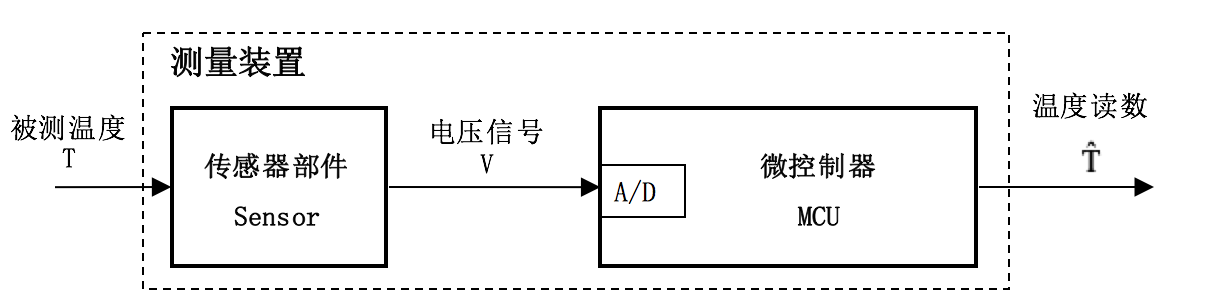
\includegraphics [scale=0.4,trim=0 0 0 0]{./image/fig1.png}
\caption{装置原理框图\citeBUAA{Paper1}}
\end{figure}
本案例的装置原理框图\citeBUAA{Paper1}如图1所示。其中,传感器部件(包括传感器元件及必要的放大电路、调理电路等)的特性是我们需要关注的重点。传感器的输入信号为被测温度,用符号$T$表示。传感器的输出信号为电压形式,用符号$V$表示。该电压信号经模数转换器(ADC)转为数字编码,被微处理器读取和程序处理,获得温度读数$\hat T$。所以,微处理器通过检测传感器电压信号,间接计算被测温度。这一操作须基于$V-\hat T$函数关系。
 
对该装置而言,标定就是指确定函数关系$\hat T = f(V)$的过程。该函数关系与传感器部件的输入输出特性$T-V$密切相关。但根据指导材料\citeBUAA{Paper1},我们可知传感器的输入输出特性具有明显的非线性和个体差异性,其$V-T$图如图2和图3所示。


我们的主要任务是找到一种合理的标定方法,使由温度预测值$\hat T$和实际值 $T$ 差异造成的误差成本最小。
\begin{figure}[H]
\centering
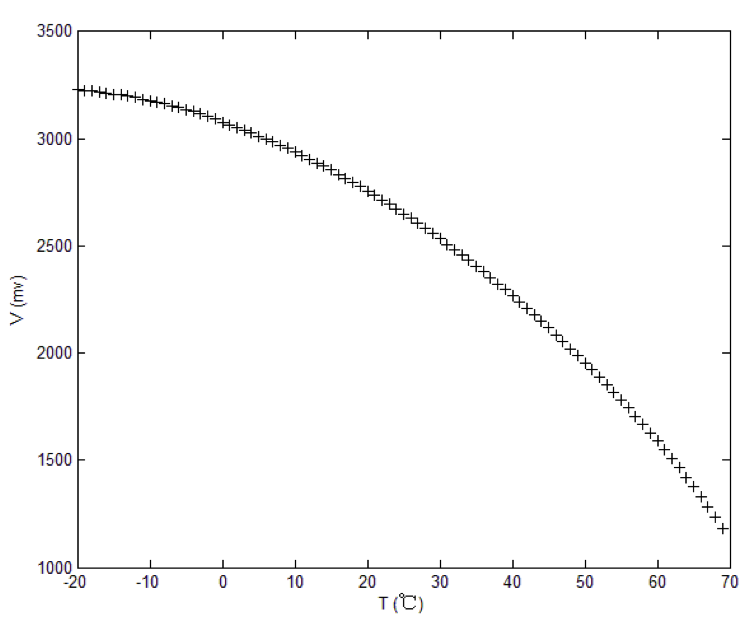
\includegraphics [scale=0.4,trim=0 0 0 0]{./image/fig2.png}
\label{fig2}
\bicaption[labelFigtu1]{图}{\centering 传感器特性的非线性}{Fig.}{\centering The non-linear property of sensors}
\end{figure}

\begin{figure}[H]
\centering
\label{fig3}
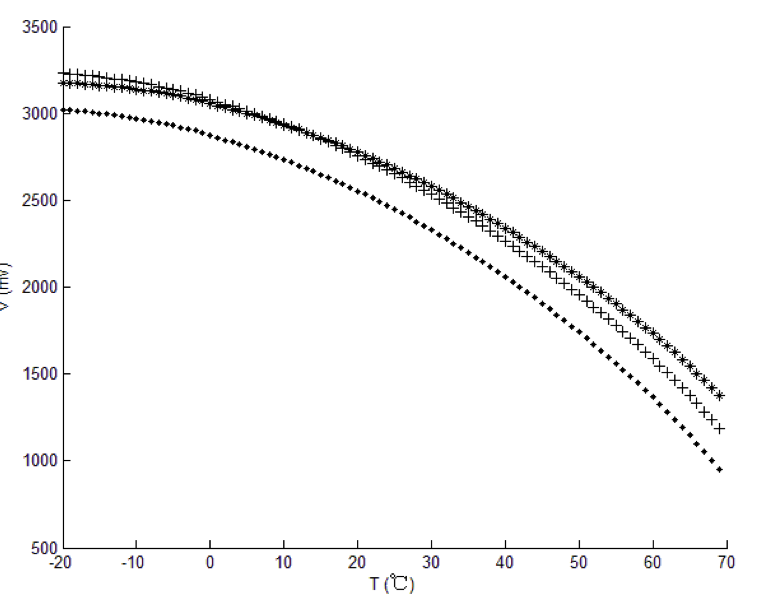
\includegraphics [scale=0.4,trim=0 0 0 0]{./image/fig3.png}
\bicaption[labelFigtu2]{图}{\centering 传感器特性的个体差异性}{Fig.}{\centering The individual difference of sensors}
\end{figure}


\subsection{标定方案评估}
根据材料\citeBUAA{Paper1},我们可以得到如下成本计算规则。
\begin{enumerate}[label=(\roman*)]
	\item \hei{单点测定成本} 
	
		\normalfont 实施一次单点测定成本记为符号$Q$, 本案例中$Q = 50$。
	\item \hei{标定误差成本}
	\normalfont
	\begin{displaymath}
			s_{i, j}=
		\begin{cases}
			0 & if\ |\hat T_{i, j} - T{i, j}| \leq 0.5 \\
			1 & if\ 0.5 < |\hat T_{i, j} - T{i, j}| \leq 1.0 \\
			4 & if\ 1.0 < |\hat T_{i, j} - T{i, j}| \leq 1.5 \\
			10 & if\ 1.5 < |\hat T_{i, j} - T{i, j}| \leq 2.0 \\
			10000 & if\ |\hat T_{i, j} - T{i, j}| > 2.0 \\
		\end{cases}
	\end{displaymath} 
	
	单点单点误差对应的成本值按上式计算,以符号$s_{i, j}$记。其中$T_{i, j}$表示第$i$个样本之第$j$点的实际温度值,$\hat T_{i, j}$表示标定后得到的估计值(读数)。
	
	单个样本个体的标定误差成本用下式计算
	
	\begin{displaymath}
		S_i = \sum_{j=1}^{90}s_{i, j}
	\end{displaymath}
	
	\item \hei{样本个体标定成本}
	\normalfont
	\begin{displaymath}
		c_i = S_i + Q \cdot n_i
	\end{displaymath}
	
	样本个体的标定成本是测定成本与误差成本之和,见上式。式中$n_i$表示对该样本个体标定过程中的测定点数目。
	\item \hei{方案成本}
	\normalfont
	标定方案的成本值按式下式计算。对标准样本库中每个样本个体逐一开展标定,取所有样本个体标定成本的统计平均。其中$M$是样本总数,$M = 500$。
	
	\begin{displaymath}
		C = \dfrac{1}{M}\sum_{i=1}^{M} c_i
	\end{displaymath}
\end{enumerate}

我们需要确定合理的采样点个数,并选择合理的采样点来进行插值处理,从而使标定方案成本最小。
\section{插值方法}
当我们确定好采样点后,我们需要选择合适的插值方法来生成电压$V$和温度预测值$\hat T$的关系曲线。性能优秀的插值方法可以减少温度预测值$\hat T$和实际值$T$的误差,从而减小标定方案的成本。因此,我们在这里介绍多项式插值、三次样条插值、$Hermite$插值法。

\subsection{多项式插值}
给定一组 $n+1$ 个数据点$(x_i,y_i)$,其中任意两个 $x_i$ 都不相同, 需要找到一个满足公式\ref{eq:1}的不大于$n$阶的$p$阶多项式。\hei 唯一性定理 \normalfont 表明存在一个并且仅有一个这样的$p$阶多项式\citeBUAA{cite1} 。

\begin{equation}
	p(x_i) = y_i, i=0,\cdots,n
	\label{eq:1}
\end{equation}

这个多项式可以表述为:对于 $n + 1$ 个插值点 ($x_i$),多项式插值定义了一个线性双射

\begin{equation}
	\bm{L}_n : \mathbb{K}^{n + 1} \rightarrow \Pi_n
\end{equation}
 
 其中$\Pi_n$ 是小于或者等于$n$的多项式的向量空间。
 构造插值多项式。。。(待续)
\subsection{三次样条插值}
对于$n+1$个给定点的数据集${x_i}$,我们可以用$n$段三次多项式在数据点之间构建一个三次样条。如公式所示,我们可以用$S(x)$来表示对函数$f$进行插值的样条函数\citeBUAA{cite2} 。
\begin{equation}
				S(x)=
		\begin{cases}
			S_0(x), & x \in [x_0,x_1] \\
			S_1(x), & x \in [x_1,x_2] \\
			 & \cdots \\
		S_{n -1}(x), & x \in [x_{n-1},x_{n}] 
		\end{cases}
\end{equation}
\begin{enumerate}[label=(\roman*)]
	\item 插值特性,$S(x_i) = f(x_i)$
	\item 样条相互连接,$S_{i-1}(x_i) = S_i(x_i), i = 1, \cdots ,n-1$
	\item 两次连续可导,$S^{\prime}_{i - 1}(x_i) = S^{\prime}_{i}(x_i)$以及$S^{\prime\prime}_{i - 1}(x_i) = S^{\prime\prime}_{i}(x_i), i = 1, \cdots , n - 1$
\end{enumerate}

由于每个三次多项式需要四个条件才能确定曲线形状,所以对于组成S的$n$个三次多项式来说,这就意味着需要$4n$个条件才能确定这些多项式。但是,插值特性只给出了$n + 1$个条件,内部数据点给出$n + 1\ −\ 2 = n\ −\ 1$个条件,总计是$4n\ −\ 2$个条件。我们还需要另外两个条件,根据不同的因素我们可以使用不同的条件。

如果令$S^{\prime}(x_0) = u\ S^{\prime}(x_k) = v$,我们可以得到$u$与$v$的钳位三次样条。特别地,当$S^{\prime\prime}(x_0) = S^{\prime\prime}(x_n) = 0$,我们得到了自然三次样条。
\subsection{$Hermite$插值}
$Hermite$插值是指在给定的节点处,不但要求插值多项式的函数值与原函数值相同。同时还要求在节点处,插值多项式的一阶直至指定阶的导数值,也与被插函数的相应阶导数值相等\citeBUAA{cite1} 。$Hermite$插值在不同的节点,提出的插值条件个数可以不同,若在某节点 $x_{i}$要求插值函数多项式的函数值,一阶导数值,直至$m_{i}-1$阶导数值均与被插函数的函数值相同及相应的导数值相等。我们称$x_{i}$为 $m_{i}$重插值点节,因此,$Hermite$插值应给出两组数,一组为插值点 $\{x_{i}\}_{i=0}^{n}$ 节点,另一组为相应的重数标号$\displaystyle \{m_{i}\}_{i=0}^{n}$。 

若 $\sum _{i=0}^{n}m_{i}=N+1$,这就说明了给出的插值条件有$N+1$个,为了保证插值多项式的存在唯一性,这时的$Hermite$插值多项式应在$P_{n}$上求得,于是可作如下定义。

$f$为$[a,b]$上充分光滑函数,对给定的插值定节 $\{x_{i}\}_{i=0}^{n}$,及相应的重数标号$\{m_{i}\}_{i=0}^{n}$,$\sum_{i=0}^n m_i = N+1$ 时,若有$H(x) \in P_{n}$满足

\begin{equation}
	H^l(x_i) = f(x_i)
\end{equation}
\begin{displaymath}
l=0,1,\ldots,m_{i-1};i=0,1,\ldots,n
\end{displaymath}
则称$H(x)$为$f(x)$关于节点$\{x_{i}\}_{i=0}^{n}$及重数标号$\{m_{i}\}_{i=0}^{n}$$\{m_{i}\}_{i=0}^{n}$的$Hermite$插值多项式。
\section{搜索算法}
根据题目数据分析,我们可知共有90个可能的温度点。根据排列组合的有关知识,我们可以得到所有的可能情况共有$2^{90}$种。这显然是令人难以接受的时间消耗,因此我们放弃暴力枚举搜索方法,转而采用启发式搜索算法。

启发式搜索算法在搜索问题解空间时,会对当前已搜索的位置进行评估,寻找认为最好的下一步搜索方向,从这个(或这些)方向进行搜索直到目标。启发式搜索可以避免简单穷举式搜索效率低的弊端(有时工作量大到无法完成)。这里我们主要介绍遗传算法和模拟退火两种启发式搜索算法。

\subsection{遗传算法}
\subsubsection{原理与基本思想}
遗传算法类似于自然进化,通过作用于染色体上的基因寻找好的染色体来求解问题。与自然界相似,遗传算法对求解问题的本身一无所知,它所需要的仅是对算法所产生的每个染色体进行评价,并基于适应值来选择染色体,使适应性好的染色体有更多的繁殖机会。在遗传算法中,通过随机方式产生若干个所求解问题的数字编码,即染色体,形成初始群体;通过适应度函数给每个个体一个数值评价,淘汰低适应度的个体,选择高适应度的个体参加遗传操作,经过遗传操作后的个体集合形成下一代新的种群。对这个新种群进行下一轮进化。这就是遗传算法的基本原理\citeBUAA{cite3} 。 

下面就是遗传算法思想:

(1) 初始化群体;    

(2) 计算群体上每个个体的适应度值;    

(3) 按由个体适应度值所决定的某个规则选择将进入下一代的个体;   

(4) 按概率$PX$进行交叉操作;   

(5) 按概率$PM$进行突变操作;    

(6) 没有满足某种停止条件,则转第(2)步,否则进入(7)。    

(7) 输出种群中适应度值最优的染色体作为问题的满意解或最优解。   

程序的停止条件最简单的有如下二种:完成了预先给定的进化代数则停止;种群中的最优个体在连续若干代没有改进或平均适应度在连续若干代基本没有改进时停止。

根据遗传算法思想,可以画出如图1所示的简单遗传算法框图。
\begin{figure}[H]
	\centering
	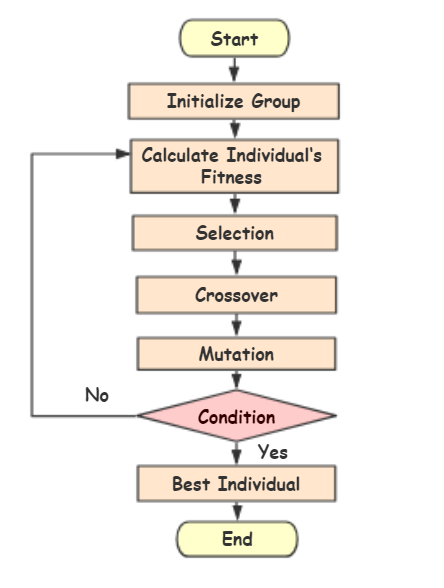
\includegraphics[scale=0.8]{./image/GA_ENG}
	\caption{遗传算法框图}
\end{figure}
\subsubsection{具体方法}

\begin{enumerate}[label = (\roman*)]

\item \hei 编码
\normalfont

编码是指把一个问题的可行解从其解空间转换到遗传算法的搜索空间的转换方法。解码(译码)是指遗传算法解空间向问题空间的转换。较好的编码应该遵守“有意义的积木块编码规则”:所定编码应当易于生成与所求问题相关的短距和低阶的积木块;最小字符集编码规则,所定编码应采用最小字符集以使问题得到自然的表示或描述。

二进制编码的缺点是汉明悬崖(Hamming Cliff),就是在某些相邻整数的二进制代码之间有很大的汉明距离,使得遗传算法的交叉和突变都难以跨越。二进制编码比十进制编码搜索能力强,但不能保持群体稳定性。
\item \hei 选择
\normalfont

遗传算法中的选择操作就是用来确定如何从父代群体中按某种方法选取那些个体遗传到下一代群体中的一种遗传运算,用来确定重组或交叉个体,以及被选个体将产生多少个子代个体。

常用的选择算子:

1、轮盘赌选择(Roulette Wheel Selection):最常用的选择算子。这是一种回放式随机采样方法。每个个体进入下一代的概率等于它的适应度值与整个种群中个体适应度值和的比例。选择误差较大。

2、随机竞争选择(Stochastic Tournament):每次按轮盘赌选择一对个体,然后让这两个个体进行竞争,适应度高的被选中,如此反复,直到选满为止。

3、最佳保留选择:首先按轮盘赌选择方法执行遗传算法的选择操作,然后将当前群体中适应度最高的个体结构完整地复制到下一代群体中。
\item \hei 交叉
\normalfont

遗传算法的交叉操作,是指对两个相互配对的染色体按某种方式相互交换其部分基因,从而形成两个新的个体。

适用于二进制编码个体或浮点数编码个体的交叉算子有如下四种:

1、单点交叉(One-point Crossover):指在个体编码串中只随机设置一个交叉点,然后再该点相互交换两个配对个体的部分染色体。

2、两点交叉(Two-point Crossover)与多点交叉(Multi-point Crossover):在个体编码串中随机设置了两个或多个交叉点,然后再进行部分基因交换。

3、均匀交叉(一致交叉,Uniform Crossover):两个配对个体的每个基因座上的基因都以相同的交叉概率进行交换,从而形成两个新个体。

4、算术交叉(Arithmetic Crossover):由两个个体的线性组合而产生出两个新的个体。该操作对象一般是由浮点数编码表示的个体。

\item \hei 变异
\normalfont

遗传算法中的变异运算,是指将个体染色体编码串中的某些基因座上的基因值用该基因座上的其它等位基因来替换,从而形成以给新的个体。

以下变异算子适用于二进制编码和浮点数编码的个体:

1、基本位变异(Simple Mutation):对个体编码串中以变异概率、随机指定的某一位或某几位仅因座上的值做变异运算。

2、均匀变异(Uniform Mutation):分别用符合某一范围内均匀分布的随机数,以某一较小的概率来替换个体编码串中各个基因座上的原有基因值。(特别适用于在算法的初级运行阶段)

3、边界变异(Boundary Mutation):随机的取基因座上的两个对应边界基因值之一去替代原有基因值。特别适用于最优点位于或接近于可行解的边界时的一类问题。
\item \hei 适应度函数
\normalfont

适应度函数也称评价函数,是根据目标函数确定的用于区分群体中个体好坏的标准。适应度函数总是非负的,而目标函数可能有正有负,故需要在目标函数与适应度函数之间进行变换。

评价个体适应度的一般过程为:1、对个体编码串进行解码处理后,可得到个体的表现型;2、由个体的表现型可计算出对应个体的目标函数值;3、根据最优化问题的类型,由目标函数值按一定的转换规则求出个体的适应度。

由目标函数$f(x)$到适应度函数$Fit[f(x)]$的转换,可以直接以待解的目标函数$f(x)$转换为适应度函数。

$Fit[f(x)]=f(x)$目标函数为最大化问题

$Fit[f(x)]=-f(x)$目标函数为最小化问题

这样处理的问题是:可能不满足常用的轮盘赌选择中概率非负的要求;某携带求解的函数在函数值分布上相差很大,由此得到的平均适应度可能不利于体现种群的平均性能。因此可以做一定的转换。

适应度尺度变换(Fitness Scaling Transform)是指在遗传算法的不同阶段,对个体的适应度进行适当的扩大或缩小。常用的尺度变换方法如下:

1、线性尺度变换:$F'=aF+b$

2、乘幂尺度变换:$F'=F^{k}$

3、指数尺度变换:$F'=exp(-\beta F)$

\item \hei 约束条件处理

\normalfont
1、搜索空间限定法:对遗传算法的搜索空间的大小加以限制,使得搜索空间中表示一个个体的点与解空间中的表示一个可行解的点有一一对应关系。

2、可行解变换法:在由个体基因型向个体表现型的变换中,增加使其满足约束条件的处理过程,即寻找个体基因型与个体表现型的多对一变换关系,扩大了搜索空间,使进化过程中所产生的个体总能通过这个变换而转化成杰空间中满足约束条件的一个可行解。

3、罚函数法:对在解空间中无对应可行解的个体计算其适应度时,处以一个惩罚函数,从而降低该个体的适应度,使该个体被遗传到下一代群体中的概率减小。
\end{enumerate}
\subsection{模拟退火算法}
模拟退火算法得益于材料的统计力学的研究成果。统计力学表明材料中粒子的不同结构对应于粒子的不同能量水平。在高温条件下,粒子的能量较高,可以自由运动和重新排列。在低温条件下,粒子能量较低。如果从高温开始,非常缓慢地降温(这个过程被称为退火),粒子就可以在每个温度下达到热平衡。当系统完全被冷却时,最终形成处于低能状态的晶体\citeBUAA{cite4} 。
如果用粒子的能量定义材料的状态,$Metropolis$算法用一个简单的数学模型描述了退火过程。假设材料在状态$i$ 之下的能量为$E(i)$,那么材料在温度$T$时从状态$i$进入状态$j$就遵循如下规律:

  (1)如果$E(j) \le E(i)$,接受该状态被转换。
  
  (2)如果$E(j) > E(i)$,则状态转换以如下概率被接受:
\begin{equation}
   p = e^{\frac{E(i)-E(j)}{KT}}
\end{equation}

其中$K$是物理学中的波尔兹曼常数$T$是材料温度。
在某一个特定温度下,进行了充分的转换之后,材料将达到热平衡。这时材料处于状态$i$的概率满足波尔兹曼分布:

\begin{equation}
P_{T}(X=i)=\frac{e^{\frac{-E(i)}{KT}}}{\underset{j \in S}{\sum} e^{\frac{-E(j)}{KT}}}
\end{equation}

其中$x$表示材料当前状态的随机变量,$S$表示状态空间集合。

显然
\begin{equation}
\underset{T\rightarrow \infty}{lim}\frac{e^{\frac{-E(i)}{KT}}}{\underset{j \in S}{\sum} e^{\frac{-E(j)}{KT}}}=\frac{1}{|S|}
\end{equation}
其中$|S|$ 表示集合$S$中状态的数量。这表明所有状态在高温下具有相同的概率。而当温度下降时,
\begin{align}
\underset{T\rightarrow 0}{lim}\frac{e^{-\frac{E(i)-E_{min}}{KT}}}{\underset{j \in S}{\sum} e^{-\frac{E(j)-E_{min}}{KT}}}=
\begin{cases}
\frac{1}{|S_{min}|}&if\ i\in S_{min}\\
0  &otherwise
\end{cases}
\end{align}
其中$E_{min}=\underset {j \in S}{min}E(j)$且$S_{min}=\{i|E(i)=E_{min}\}$。
上式表明当温度降至很低时,材料会以很大概率进入最小能量状态。
假定我们要解决的问题是一个寻找最小值的优化问题。将物理学中模拟退火的思想应用于优化问题就可以得到模拟退火寻优方法。
考虑这样一个组合优化问题:优化函数为$f:\rightarrow R^{+}$,其中$x\in S$,它表示优化问题的一个可行解,$R^{+}=\{y|y>0\}$,$S$表示函数的定义域。$N(x)\subset S$表示$x$的一个邻域集合。

首先给定一个初始温度$T_{i}$ 和该优化问题的一个初始解$x(k)$,并由$x(0)$ 生成下一个解$x'\in N(x(0))$,是否接受$x'$作为一个新解$x(k+1)$ 依赖于下面概率:
\begin{align}
P(x(k)\rightarrow x')=\begin{cases}
1 &if\ f(x')<f(x(k))\\
e^{-\frac{f(x')-f(x(k))}{T_{i}}} &otherwise
\end{cases}
\end{align}
在温度$T_{i}$ 下,经过很多次的转移之后,降低温度$T_{i}$ ,得到$T_{i+1} <T_{i}$。在$T_{i}$下重复上述过程。因此整个优化过程就是不断寻找新解和缓慢降温的交替过程。最终的解是对该问题寻优的结果。
我们注意到,在每个$T_{i}$下,所得到的一个新状态$x(k+1)$完全依赖于前一个状态$x(k)$ ,可以和前面的状态 $x(0),x(1),……,x(k-1)$无关,因此这是一个马尔可夫过程。使用马尔可夫过程对上述模拟退火的步骤进行分析,结果表明:从任何一个状态$x(k)$生成$x'$的概率,在$N(x(k))$中是均匀分布的,且新状态$x'$被接受的概率满足式$(3)$那么经过有限次的转换,在温度$T_{i}$下的平衡态$x_{i}$的分布由下式给出:
\begin{equation}
P_{i}(T_{i})=\frac{e^{-\frac{f(x_{i})}{T_{i}}}}{\underset{j\in S}{\sum}e^{-\frac{f(x_{j})}{T_{i}}}}
\end{equation}
  当温度$T_{i}$降为0时,$x_{i}$的分布为:
\begin{equation}
P_{i}^{*}=\begin{cases}
\dfrac{1}{|S_{min}|}&if\ x_{i}\in S_{min}\\
0 & otherwise
\end{cases}
\end{equation}
  并且:
\begin{equation}
\underset{x_{i}\in S_{min}}{\sum}P_{i}^{*}=1
\end{equation}
  这说明如果温度下降十分缓慢,而在每个温度都有足够多次的状态转移,使之在每一个温度下达到热平衡,则全局最优解将以概率 1 被找到。因此可以说模拟退火算法可以找到全局最优解。在模拟退火算法中应注意以下问题:
 \begin{enumerate}[label=(\alph*) ]
 	\item 理论上,降温过程要足够缓慢,要使得在每一温度下达到热平衡。但在计算机实现中,如果降温速度过缓,所得到的解的性能会较为令人满意,但是算法会太慢,相对于简单的搜索算法不具有明显优势。如果降温速度过快,很可能最终得不到全局最优解。因此使用时要综合考虑解的性能和算法速度,在两者之间采取一种折衷。
 	\item 确定在每一温度下状态转换的结束准则。实际操作可以考虑当连续$m$次的转换过程没有使状态发生变化时结束该温度下的状态转换。最终温度的确定可以提前定$t_{E}$为一个较小的值,或连续几个温度下转换过程没有使状态发生变化算法就结束。
 	\item 选择初始温度和确定某个可行解的邻域的方法也要恰当。
 \end{enumerate}
\section{模型构建}
在模型构建中,我们分别采用遗传算法和模拟退火算法作为遗传算法,尝试不同的插值方法,寻找最低平均成本的标定方案。
\subsection{基于遗传算法的标定模型}
\begin{enumerate}[label=(\roman*)]
	\item \hei 编码

	\normalfont 由于测试温度点共有90个,每个温度点均有两种可能:选择作为采样点或者不选择。因此,我们可以考虑在编码过程中采用二进制编码。每个个体有长度为90的二进制基因序列,基因序列中的每个基因点对应着一个特定的温度点。我们不妨设基因序列为$Gene$,其起点为$Gene[1]$,终点为$Gene[90]$。因此我们可以得到$Gene[i] = 1, 
	\cdots , n$的解析式。
	
	\begin{equation}
		Gene[i]=
		\begin{cases}
			0 & \text{该温度点不被选取}\\
			1 & \text{该温度点被选取}
		\end{cases}
	\end{equation}
	
	同时,我们给出基因序列$Gene$的序号$index$和温度点$T$的数值对应关系式。
	
	\begin{equation}
		index = T + 21
	\end{equation}
	
\item \hei 选择
\normalfont

在选择过程中,我们一开始采用轮盘赌选择(Roulette Wheel Selection)方法。但是通过追踪实验结果,我们发现在迭代过程中会存在由于变异丢失种群最优解的现象。因此,我们决定采用最佳保留选择法。首先我们执行轮盘赌选择方法,并记录选择之前的当前种群最优个体。选择过程结束后,我们将当前种群的最优个体完整地复制到了下一代的种群中。

最佳保留选择法有效地保护了当前种群的最优个体,避免了由于突变所造成的最优个体丢失。这保证了在迭代过程中的当前最优解会一直保持在最优状态,不会出现\kai{退化现象}。
\item \hei 交叉
\normalfont

在交叉过程中,我们采用单点交叉。我们利用生成$1-90$的随机数,然后以该点作为交叉点。交叉点及其以前的基因序列与父代相同,交叉点及其以后的基因序列与母带相同。
\item \hei 变异
\normalfont

在变异过程中,由于二进制编码的天然特点,我们选择基本位变异。在试验的开始阶段,我们选择单点变异。但经过实验发现,单点变异对在该案例中对寻找最终优化结果帮助很小。所以,我们尝试提高变异概率和增加变异点个数。结果表明,该案例对应的遗传性能有显著提高。
\item \hei 适应度函数
\normalfont

在评价个体的适应度过程中,我们很容易得到如下关系:

\kai 个体适应度随着标定方案成本的升高而降低。

\normalfont 因此当给定基因序列$Gene$时,我们可以根据对应的插值方法,计算出$V-\hat T$曲线。并根据上文中的评估方案,得到方案成本$C(Gene)$。由于该问题为目标函数$C(Gene)$最小化问题,所以我们可以得出适应度函数$Fit[C(Gene)]$的如下解析式:
\begin{equation}
	Fit[C(Gene)] = - C(Gene)
\end{equation}
\end{enumerate}



\section{结果分析}
\subsection{基于遗传算法的标定模型}
首先,我们比较在其他条件完全相同的情况下,采用不同的插值方法所得到的最优结果。

其次,我们探究突变概率和突变点个数对算法性能的影响。

最后,我们给出经过优化调节参数后所能得到的最优解。
\begin{flushleft}
	\kai 
选择1,5,14,17,19,20,21,22,24,28,39,55,72,82,88,90共16个温度点。(第$i$个温度点对应的温度为$i - 21$) 所求得的最低成本为800.212元。
\end{flushleft}
\vspace{1em}

{\hei\wuhao 致谢\quad}
{\fang\wuhao 
感谢蒋乐天老师对我们的悉心指导,帮助我们较为顺利地完成了本次案例论文的书写和代码的编写。
}
\section{未来工作}
在十一期间,我们已经开展了较为有效的小组学习。自学了遗传算法和模拟退火算法的算法原理,并且分别用Python和Matlab实现了基于遗传的算法标定模型。

我们初步利用该模型,求解到了当前最优值800.202元。在参数调定和代码编写的过程中,我们掌握到了许多Matlab编程的技巧同时感受了面向对象强大的威力。

在我们未来的工作中,我们会进一步完善遗传算法。探索除三次样条差值方法,其他方法求解答得到的最优化结果。我们在实验中发现突变过程,对本题中的求解影响很大。我们未来会进一步探索突变概率和突变点个数对遗传算法算法性能的影响。

我们也会尝试模拟退火算法,利用其建立基于模拟退火算法的标定模型。并最终根据相关参数,求解最优化问题。

这是我们小组近期的规划。


%%%%%%%%%%%%%%%%%%%%%%%%%%%%%%%%%%%%%%%%%%%%%%%%%%%%%%%%%%%%%%%%
%  参考文献
%%%%%%%%%%%%%%%%%%%%%%%%%%%%%%%%%%%%%%%%%%%%%%%%%%%%%%%%%%%%%%%%
\renewcommand\refname{\hei\wuhao\centerline{参考文献(References)}\global\def\refname{参考文献}}
\vskip 12pt

\let\OLDthebibliography\thebibliography
\renewcommand\thebibliography[1]{
  \OLDthebibliography{#1}
  \setlength{\parskip}{0pt}
  \setlength{\itemsep}{0pt plus 0.3ex}
}

{
\renewcommand{\baselinestretch}{0.9}
\liuhao
\bibliographystyle{unsrt}
\bibliography{./TempExample}
}
%%%%%!!!!!需要在合适位置插入\newpage,来平衡最后一页两栏!!!!!
\newpage  %%% 用于平衡最后一页两栏高度

%%%%%%%%%%%%%%%%%%%%%%%%%%%%%%%%%%%%%%%%%%%%%%%%%%%%%%%%%%%%%%%
% % % 附录
%%%%%%%%%%%%%%%%%%%%%%%%%%%%%%%%%%%%%%%%%%%%%%%%%%%%%%%%%%%%%%%
\twocolumn[
\begin{@twocolumnfalse}
\vskip 20pt
 
 \noindent {\hei 附录A:基于遗传算法的标定方案代码实现}
 \newline
 \kai (1) 个体(Chromosome)类的设计
\lstinputlisting{Chromosome.m}
\end{@twocolumnfalse}
]
\twocolumn[
\begin{@twocolumnfalse}
\kai(2)种群(Population)类的设计
\lstinputlisting{Population1.m}
\end{@twocolumnfalse}
]
\twocolumn[
\begin{@twocolumnfalse}
\lstinputlisting{Population2.m}

\end{@twocolumnfalse}
]

\twocolumn[
\begin{@twocolumnfalse}
\lstinputlisting{Population3.m}
\kai(3)在给定参数的条件下,求解最优测定方案
\lstinputlisting{GA.m}
 \noindent {\hei 附录B:基于模拟退火算法的标定方案代码实现}

\end{@twocolumnfalse}
]
\end{document}
 